\section{Hai đường thẳng vuông góc}

\subsection{Đề 1}
\Opensolutionfile{ans}[ans/ans-1-C8B1]
\caulc

%%%==============Câu_1============%%%
\begin{ex}%[1H8N1-1] 
Trong không gian cho điểm $A$ và đường thẳng $d$. Có bao nhiêu đường thẳng qua $A$ và vuông góc với đường thẳng $d$?
	\choice
		{$0$}
		{$1$}
		{$2$}
		{\True Vô số}
	\loigiai{
		Có vô số đường thẳng qua $A$ và vuông góc với đường thẳng $d$.
		}
\end{ex}

%%%==============Câu_2============%%%
\begin{ex}%[1H8H1-1] 
Trong không gian cho ba đường thẳng phân biệt $a$, $b$, $c$. Khẳng định nào sau đây đúng?
	\choice
		{Nếu đường thẳng $a$ vuông góc với đường thẳng $b$ và đường thẳng $b$ vuông góc với đường thẳng $c$ thì đường thẳng $a$ vuông góc với đường thẳng $c$}
		{\True Nếu đường thẳng $a$ vuông góc với đường thẳng $b$ và đường thẳng $b$ song song với đường thẳng $c$ thì đường thẳng $a$ vuông góc với đường thẳng $c$}
		{Trong không gian, nếu đường thẳng $a$ song song với đường thẳng $b$ và đường thẳng $b$ vuông góc với đường thẳng $c$ thì đường thẳng $a$ cắt đường thẳng $c$ tại một điểm}
		{Nếu ba đường thẳng $a$, $b$, $c$ vuông góc với nhau từng đôi một và có đường thẳng $d$ vuông góc với đường thẳng $a$ thì đường thẳng $d$ song song với $b$ hoặc $c$}
	\loigiai{
		Theo cách xác định góc giữa hai đường thẳng trong không gian, vì $b \parallel c$ nên ta có $(a,b)=(a,c)=90^\circ$ hay $a \perp c$. Suy ra chọn đáp án B.}
\end{ex}

%%%==============Câu_3============%%%
\begin{ex}%[1H8H1-1] 
Trong các mệnh đề sau, mệnh đề nào sai?
	\choice
		{\True Hai đường thẳng phân biệt cùng vuông góc với một đường thẳng thứ ba thì song song với nhau}
		{Hai đường thẳng phân biệt cùng song song với một đường thẳng thì song song với nhau}
		{Một đường thẳng vuông góc với hai cạnh của tam giác thì sẽ vuông góc với cạnh thứ ba của tam giác đó}
		{Hai đường thẳng vuông góc nếu góc giữa hai véc tơ chỉ phương của chúng bằng $90^\circ$}
	\loigiai{
		Hai đường thẳng phân biệt cùng vuông góc với đường thẳng thứ ba có thể song song, cắt nhau hoặc chéo nhau.
		}
\end{ex}

%%%==============Câu_4============%%%
\begin{ex}%[1H8N1-3]
\immini{Cho hình chóp $S.ABCD$ có đáy $ABCD$ là hình bình hành. Góc giữa hai đường thẳng $SD$ và $BC$ bằng
\choice
		{Góc giữa hai đường $SD$ thẳng và $CD$}
		{\True Góc giữa hai đường thẳng $SD$ và $AD$}
		{Góc giữa hai đường thẳng $SD$ và $BD$}
		{Góc giữa hai đường thẳng $SD$ và $SC$}
}{
    {\begin{tikzpicture}[scale=1, font=\footnotesize, line join=round, line cap=round, >=stealth]
	\def\a{2} \def\b{3} \def\h{2.5}
	\path
	(0:0) coordinate (A)
		(0:\b) coordinate (D)
		(-140:\a) coordinate (B)
		($(B)+(D)-(A)$) coordinate (C)
		($(A)+(70:\h)$) coordinate (S);
		\draw (D)--(C)--(B)--(S)--(C) (S)--(D);
		\draw[dashed] (S)--(A)--(B) (A)--(D);
		\foreach \x/\g in {A/180,B/-90,C/-90,D/0,S/90}
		\fill[black] (\x) circle(1pt) ($(\x)+(\g:3mm)$) node{$\x$};
		\end{tikzpicture}}
}
	\loigiai{
		Do $BC \parallel AD$ nên góc giữa hai đường thẳng $SD$ và $BC$ bằng góc giữa hai đường thẳng $SD$ và $AD$.
		}
\end{ex}

%%%==============Câu_5============%%%
\begin{ex}%[1H8N1-3]
\immini{
Cho hình lập phương $ABCD.A'B'C'D'$. Góc giữa hai đường thẳng $BD$ và $A'C'$ bằng
	\choice
		{\True Góc giữa hai đường thẳng $BD$ và $AC$}
		{Góc giữa hai đường thẳng $BD$ và $B'D'$}
		{Góc giữa hai đường thẳng $BD$ và $A'B'$}
		{Góc giữa hai đường thẳng $BD$ và $AC'$}
}{
\begin{tikzpicture}[scale=1, font=\footnotesize, line join=round, line cap=round, >=stealth]
				\def\a{1.6} \def\b{2.6} \def\h{2} \def\g{-120}
				\path
				(0:0) coordinate (A)
				(\g:\a) coordinate (B)
				(0:\b) coordinate (D)
				($(B)+(D)-(A)$) coordinate (C)
				;
				\foreach \x in {A,B,C,D} \coordinate (\x') at ($(\x)+(90:\h)$);
				\draw (B')--(A')--(D')--(C')--(B')--(B)--(C)--(D)--(D') (C)--(C');
				\draw[dashed] (B)--(A)--(D) (A)--(A');
				\foreach \i/\g in {A/-80,B/-90,C/-90,D/0,A'/90,D'/90,B'/180,C'/110}
				\fill[black] (\i) circle(1pt) ($(\i)+(\g:3mm)$) node{$\i$};
	\end{tikzpicture}
}
	\loigiai{
		Do $AC \parallel A'C'$ nên góc giữa hai đường thẳng $BD$ và $A'C'$ bằng góc giữa hai đường thẳng $BD$ và $AC$.
		}
\end{ex}

%%%==============Câu_6============%%%
\begin{ex}%[1H8N1-3]
\immini{
Cho hình chóp $S.ABCD$ có tất cả các cạnh bằng nhau. Góc giữa hai đường thẳng $SA$ và $CD$ bằng
	\choice
		{Góc giữa hai đường thẳng $SA$ và $BD$}
		{\True Góc giữa hai đường thẳng $SA$ và $AB$}
		{Góc giữa hai đường thẳng $SA$ và $SC$}
		{Góc giữa hai đường thẳng $SA$ và $AC$}
}{
\begin{tikzpicture}[scale=1, font=\footnotesize, line join=round, line cap=round, >=stealth]
	\def\a{2} \def\b{3} \def\h{2.5}
	\path
	(0:0) coordinate (A)
		(0:\b) coordinate (D)
		(-140:\a) coordinate (B)
		($(B)+(D)-(A)$) coordinate (C)
		($(A)+(70:\h)$) coordinate (S);
		\draw (D)--(C)--(B)--(S)--(C) (S)--(D);
		\draw[dashed] (S)--(A)--(B) (A)--(D);
		\foreach \x/\g in {A/180,B/-90,C/-90,D/0,S/90}
		\fill[black] (\x) circle(1pt) ($(\x)+(\g:3mm)$) node{$\x$};
		\end{tikzpicture}
}
	\loigiai{
		Do $AB \parallel CD$ nên góc giữa hai đường thẳng $SA$ và $CD$ bằng góc giữa hai đường thẳng $SA$ và $AB$.
		}
\end{ex}

%%%============Câu_7==============%%%
\begin{ex}%[1H8H1-3]
\immini{
Cho hình chóp $S.ABCD$ có tất cả các cạnh bằng nhau (hình vẽ minh hoạ). Số đo góc giữa hai đường thẳng $SA$ và $BC$ bằng
	\choice
		{$90^\circ$}
		{\True $60^\circ$}
		{$45^\circ$}
        {$30^\circ$}
}{
\begin{tikzpicture}[scale=1, font=\footnotesize, line join=round, line cap=round, >=stealth]
	\def\a{2} \def\b{3} \def\h{2.5}
	\path
	(0:0) coordinate (A)
		(0:\b) coordinate (D)
		(-140:\a) coordinate (B)
		($(B)+(D)-(A)$) coordinate (C)
		($(A)+(70:\h)$) coordinate (S);
		\draw (D)--(C)--(B)--(S)--(C) (S)--(D);
		\draw[dashed] (S)--(A)--(B) (A)--(D);
		\foreach \x/\g in {A/180,B/-90,C/-90,D/0,S/90}
		\fill[black] (\x) circle(1pt) ($(\x)+(\g:3mm)$) node{$\x$};
		\end{tikzpicture}
}
\loigiai{
 $S.ABCD$ có tất cả các cạnh bằng nhau suy ra $\triangle SAD$ đều.\\
 Khi đó $BC \parallel AD$ $\Rightarrow$ $(SA;BC)=(SA;AD)=\widehat{SAD}=60^\circ$ 
    }
\end{ex}

%%%==============Câu_8============%%%
\begin{ex} %[1H8N1-3]
\immini{
Cho hình lập phương $ABCD.A'B'C'D'$. Góc giữa hai đường thẳng $AA'$ và $DC'$ bằng
	\choice
		{Góc giữa hai đường thẳng $AA'$ và $DD'$}
		{Góc giữa hai đường thẳng $AA'$ và $D'C'$}
		{Góc giữa hai đường thẳng $DD'$ và $BB'$}
		{\True Góc giữa hai đường thẳng $DC'$ và $DD'$}
}{
\begin{tikzpicture}[scale=1, font=\footnotesize, line join=round, line cap=round, >=stealth]
				\def\a{1.6} \def\b{2.6} \def\h{2} \def\g{-120}
				\path
				(0:0) coordinate (A)
				(\g:\a) coordinate (B)
				(0:\b) coordinate (D)
				($(B)+(D)-(A)$) coordinate (C)
				;
				\foreach \x in {A,B,C,D} \coordinate (\x') at ($(\x)+(90:\h)$);
				\draw (B')--(A')--(D')--(C')--(B')--(B)--(C)--(D)--(D') (C)--(C');
				\draw[dashed] (B)--(A)--(D) (A)--(A');
				\foreach \i/\g in {A/-80,B/-90,C/-90,D/0,A'/90,D'/90,B'/180,C'/110}
				\fill[black] (\i) circle(1pt) ($(\i)+(\g:3mm)$) node{$\i$};
	\end{tikzpicture}
}
\loigiai{
    Do $AA' \parallel DD'$ nên góc giữa hai đường thẳng $AA'$ và $DC'$ bằng góc giữa hai đường thẳng $DD'$ và $DC'$.}
\end{ex}

%%%==============Câu_9============%%%
\begin{ex}%[1H8V1-3]
\immini
{Cho hình lập phương $ABCD.A'B'C'D'$. Góc giữa hai đường thẳng $AC$ và $A'D$ là
	\choice
		{$90^\circ$}
		{\True $0^\circ$}
		{$45^\circ$}
        {$120^\circ$}
}
{\begin{tikzpicture}[scale=1, font=\footnotesize, line join=round, line cap=round, >=stealth]
				\def\a{1.2} \def\b{2.4} \def\h{2} \def\g{-110}
				\path
				(0:0) coordinate (A)
				(\g:\a) coordinate (B)
				(0:\b) coordinate (D)
				($(B)+(D)-(A)$) coordinate (C)
				;
				\foreach \x in {A,B,C,D} \coordinate (\x') at ($(\x)+(90:\h)$);
				\draw (B')--(A')--(D')--(C')--(B')--(B)--(C)--(D)--(D') (C)--(C') (D)--(C') (A')--(C') ;
				\draw[dashed] (B)--(A)--(D) (A)--(A') (A)--(C) (A')--(D);
				\foreach \i/\g in {A/180,B/-90,C/-90,D/0,A'/90,D'/90,B'/180,C'/110}
				\fill[black] (\i) circle(1pt) ($(\i)+(\g:3mm)$) node{$\i$};
	\end{tikzpicture}}
	\loigiai{
		Vì $A'C' \parallel AC$ nên góc giữa $AC$ và $A'D$ bằng góc giữa hai đường thẳng $A'C'$ và $A'D$.
		Vì tam giác $A'C'D$ đều nên $\widehat{AD'C'}=60^\circ$.\\
        Vậy góc giữa $AC$ và $A'D$ bằng $60^\circ$.
		}
\end{ex}

%%%==============Câu_10============%%%
\begin{ex}%[1H8H1-1]
Mệnh đề nào dưới đây là đúng?
	\choice
		{Nếu một đường thẳng vuông góc với một trong hai đường thẳng song song thì cũng vuông góc với đường thẳng còn lại}
		{Hai đường thẳng vuông góc với nhau thì luôn cắt nhau}
		{Góc giữa hai đường thẳng bằng góc giữa hai vec-tơ chỉ phương của chúng}
		{\True Hai đường thẳng cùng vuông góc với một đường thẳng thì song song với nhau}
	\loigiai{
		\begin{itemchoice}
			\itemch Đúng. Giả sử $a \perp b$ và $b \parallel c$ thì $(a,b)=(a,c)=90^\circ$, vậy $a \perp c$.
			\itemch Sai vì hai đường thẳng vuông góc có thể chéo nhau.
			\itemch Sai vì góc giữa hai đường thẳng luôn nhỏ hơn hoặc bằng còn góc giữa hai vectơ có thể là góc tù.
			\itemch Sai vì hai đường thẳng cùng vuông góc với một đường thẳng thì có thể cắt nhau.
		\end{itemchoice}
		}
\end{ex}

%%%==============Câu_11============%%%
\begin{ex}%[1H8V1-3]
Cho tứ diện $ABCD$ có $AB=CD=2a$. Gọi $M$, $N$ lần lượt là trung điểm của $BC$, $AD$. Biết rằng $MN=a\sqrt{3}$. Tính góc giữa hai đường thẳng $AB$ và $CD$.
	\choice
		{$45^\circ$}
		{$30^\circ$}
		{$90$}
		{\True $60$}
	\loigiai{
        \immini
        {Gọi $I$ là trung điểm của $AC$. Ta có $IM=IN=a$.\\
        Áp dụng định lý cosin cho $\triangle IMN$, ta có
        $$ \cos{MIN} =\dfrac{IM^2+IN^2-MN^2}{2\cdot IM \cdot IN}= \dfrac{a^2+a^2-3a^2}{2\cdot a\cdot a}=\dfrac{1}{2}.$$
        Suy ra $\widehat{MIN}=120^\circ$ .\\    Vì $IM \parallel AB$ và $IN \parallel CD$,\\
        nên $(AB,CD)=(IM,IN)=180^\circ-120^\circ=60^\circ$.   
        }
        {\begin{tikzpicture}[scale=1, font=\footnotesize, line join=round, line cap=round, >=stealth]
				\def\a{3.5} \def\b{1.8} \def\h{2.7}
				\path
				(0:0) coordinate (C)
				(0:\a) coordinate (D)
				(-60:\b) coordinate (B)
				($(C)+(70:\h)$) coordinate (A)
				($(A)!1/2!(D)$) coordinate (N)
                ($(C)!1/2!(B)$) coordinate (M)
				($(A)!1/2!(C)$) coordinate (I);
				\draw (A)--(C)--(B)--(D)--(A)--(C) (A)--(B) (M)--(I);
				\draw[dashed] (C)--(D) (M)--(N)--(I);
				\foreach \x/\g in {A/90,C/180,B/-90,D/0,N/0,M/180,I/180}
				\fill[black] (\x) circle(1pt) ($(\x)+(\g:3mm)$) node{$\x$};
			\end{tikzpicture}}
		}
\end{ex}

%%%==============Câu_12============%%%
\begin{ex}%[1H8V1-3]
    Cho hình chóp $S.ABCD$ có tất cả các cạnh đều bằng $a$, $O$ là tâm hình vuông $ABCD$. Gọi $M$, $N$ lần lượt là trung điểm $AB$ và $SB$. Gọi $\alpha$ là góc giữa hai đường thẳng $MN$ và $MO$. Khi đó $\cos\alpha$ bằng
    \choice
    {$\dfrac{\sqrt{3}}{2}$}
    {\True $\dfrac{1}{2}$}
    {$\dfrac{\sqrt{2}}{2}$}
    {$\dfrac{\sqrt{3}}{6}$}
    \loigiai{
    \immini
    {Hình chóp $S.ABCD$ có tất cả các cạnh đều bằng $a$ suy ra $\triangle SAD$ đều và $(SA,AD)=60^\circ$.\\
    Mặt khác ta có $SA \parallel MN$ và $AD \parallel MO$.\\
    $\Rightarrow
    \alpha=(MN,MO)=(SA,AD)=60^\circ$.\\
    Vậy $\cos{\alpha}=\dfrac{1}{2}$.}
    {\begin{tikzpicture}[line join=round,line cap=round,line width=.6pt,font=\footnotesize,scale=1]
	\coordinate[label=below left:$B$] (B) at (0,0);
	\coordinate[label=above right:$A$] (A) at (2,1);
	\coordinate[label=below right:$C$] (C) at (5,0);
	\coordinate[label=above right:$D$] (D) at ($(C)-(B)+(A)$);
	\coordinate[label=below:$O$] (O) at ($(A)!.5!(C)$);
	\coordinate[label=above left:$S$] (S) at ($(O)+(90:4)$);
	\coordinate[label= left:$M$] (M) at ($(A)!.5!(B)$);
        \coordinate[label= left:$N$] (N) at ($(S)!.5!(B)$);
	\draw (B)--(C)--(D)--(S)--cycle (S)--(C);
	\draw[dashed] (C)--(A)--(D)--(B) (O)--(S)--(A)--(B) (N)--(O)--(M)--(N);
	\fill (A)circle(1.5pt) (B)circle(1.5pt) (C)circle(1.5pt)(M)circle(1.5pt) (D)circle(1.5pt) (S)circle(1.5pt) (O)circle(1.5pt);
\end{tikzpicture}}
    }
\end{ex}

\Closesolutionfile{ans}
\indapan{6}{ans/ans-1-C8B1}

\cauds
\Opensolutionfile{ans}[ans/ans-1-C8B1-DS]
%%%==============Cau_1============%%%
\begin{ex}%[1H8N1-1]
	Trong không gian, cho ba đường thẳng phân biệt. Xác định tính đúng sai các mệnh đề sau?
	\choiceTF
%	[t]
		{\True Nếu $a \parallel b$ thì $(a,c)=(c,b)$}
		{\True Nếu $c \parallel b$ thì $(a,b)=(a,c)$}
		{Nếu $a \perp c$, $b \perp c$ thì $a \parallel b$}
		{Nếu $a \perp c$ thì $(a,b)=(c,b)$}
	\loigiai{
		\begin{itemchoice}
	\itemch Đúng vì theo định nghĩa góc giữa hai đường thẳng trong không gian là góc giữa đường thẳng lần lượt song song hoặc trùng với chúng.
	\itemch Đúng vì theo định nghĩa góc giữa hai đường thẳng trong không gian là góc giữa đường thẳng lần lượt song song hoặc trùng với chúng.
	\itemch Sai vì $a$ và $b$ có thể chéo nhau.
	\itemch Sai vì theo định nghĩa góc giữa hai đường thẳng trong không gian là góc giữa đường thẳng lần lượt song song hoặc trùng với chúng.   
		\end{itemchoice}}
\end{ex}

%%%==============Cau_2============%%%
\begin{ex}%[1H8V1-3] 
	Cho hình lập phương $ABCD.A'B'C'D'$. Xét tính đúng sai của các khẳng định sau:
	\choiceTF
%	[t]
		{\True $BD \parallel B'D'$}
        {\True $(AC,B'D')=90^\circ$}
		{\True Tam giác $ACD'$ đều}
		{$(AC,A'B)=30^\circ$}
	\loigiai{
        \begin{center}
        \begin{tikzpicture}[scale=1, font=\footnotesize, line join=round, line cap=round, >=stealth]
				\def\a{1.6} \def\b{3} \def\h{2.5} \def\g{-110}
				\path
				(0:0) coordinate (A)
				(\g:\a) coordinate (B)
				(0:\b) coordinate (D)
				($(B)+(D)-(A)$) coordinate (C)
				;
				\foreach \x in {A,B,C,D} \coordinate (\x') at ($(\x)+(90:\h)$);
				\draw (B')--(A')--(D')--(C')--(B')--(B)--(C)--(D)--(D') (C)--(C') (D')--(C) (B')--(D');
				\draw[dashed] (B)--(A)--(D) (A)--(A')--(B) (A)--(C) (B)--(D) (A)--(D');
				\foreach \i/\g in {A/-80,B/-90,C/-90,D/0,A'/90,D'/90,B'/180,C'/110}
				\fill[black] (\i) circle(1pt) ($(\i)+(\g:3mm)$) node{$\i$};
	\end{tikzpicture}\end{center}
        \begin{itemchoice}
        \itemch Đúng.\\
        Ta có $BB' \parallel DD'$ và $BB' = DD'$.\\
        $\Rightarrow$ $BDD'B'$ là hình bình hành $\Rightarrow BD \parallel B'D'$.
        \itemch Đúng.\\
        Vì $BD \parallel B'D' \Rightarrow (AC,B'D')=(AC,BD)=90^\circ$ (do $ABCD$ là hình vuông).
        \itemch Đúng.\\
        Ta có $A'D' \parallel BC$, $A'D' = BC$\\
        $\Rightarrow$
        $ABCD$ là hình bình hành $\Rightarrow AB \parallel CD$.\\
        Vì vậy $(AC,A'B)=(AC,CD)$.\\
        Gọi $a$ là cạnh của hình lập phương thì $AD'=CD'=AC=a\sqrt{2}$ (đường chéo của hình vuông cạnh $a$).\\
        Suy ra tam giác $ACD'$ đều.
        \itemch Sai.\\
        Tam giác $ACD'$ đều nên $(AC, CD')=\widehat{ACD}=60^\circ$.\\
    Vậy $(AC,A'B)=60^\circ$.
         \end{itemchoice}}
\end{ex}

%%%==============Cau_3============%%%
\begin{ex}%[1H8V1-3] 
    Cho hình chóp $S.ABCD$ có đáy là hình thoi. Gọi $M, N$ lần lượt là trung điểm củac các đoạn thẳn $SB, SD$. Xét tính đúng sai của các khẳng định sau:
    \choiceTF
%    [t]
        {\True $MN \parallel BD$}
        {\True $MN$ và $AC$ là hai đường thẳng chéo nhau}
        {\True $AC\perp BD$}
        {\True $(MN,AC)=90^\circ$}
    \loigiai{
    	\begin{center}
    	\begin{tikzpicture}[scale=1, font=\footnotesize, line join=round, line cap=round, >=stealth]
    		\def\a{2} \def\b{3} \def\h{2.5}
    		\path
    		(0:0) coordinate (A)
    		(0:\b) coordinate (D)
    		(-130:\a) coordinate (B)
    		($(B)+(D)-(A)$) coordinate (C)
    		($(A)+(80:\h)$) coordinate (S)
    		($(A)!1/2!(C)$) coordinate (O)
    		($(S)!1/2!(B)$) coordinate (M)
    		($(S)!1/2!(D)$) coordinate (N);
    		\draw (D)--(C)--(B)--(S)--(C) (S)--(D);
    		\draw[dashed] (S)--(A)--(B) (C)--(A)--(D)--(B) (M)--(N) (S)--(O);
    		\foreach \x/\g in {A/180,B/-90,C/-90,D/0,S/90,O/-90,M/180,N/0}
    		\fill[black] (\x) circle(1pt) ($(\x)+(\g:3mm)$) node{$\x$};
    	\end{tikzpicture}
    	\end{center}
		\begin{itemchoice}
        \itemch Đúng.\\
        $M, N$ lần lượt là trung điểm củac các đoạn thẳn $SB, SD$.\\
        $\Rightarrow$ $MN$ là đường trung bình của tam giác $SBD$.\\
        $\Rightarrow$ $MN \parallel BD$.
        \itemch Đúng.\\
        $MN \parallel BD$ nên $MN \parallel (ABCD)$.\\
        Mà $AC$ và $BD$ cắt nhau.\\
        Vậy $MN$ và $AC$ chéo nhau.
        \itemch Đúng.\\
        $ABCD$ là hình thoi nên $AC \perp BD$.
        \itemch Đúng.\\
        $ABCD$ là hình thoi nên $(AC,BD)=90^\circ$.\\
        $MN \parallel BD$ nên $(MN,AC)=(BD,AC)=90^\circ$.
    	\end{itemchoice}}
\end{ex}

%%%==============Cau_4============%%%
\begin{ex} %[1H8V1-3] 
    Cho tứ diện đều $ABCD$ có cạnh bằng $a$, $M$ là trung điểm cạnh $BC$, $N$ là trung điểm của $AC$. Xét tính đúng sai của các khẳng định sau:
    \choiceTF
%    [t]
        {\True $MN \parallel AB$}
        {$MN=ND=\dfrac{a\sqrt{2}}{2}$}
        {\True $(AB, MD)=(MN, MD)$}
        {$\cos{(AB,MD)}=\dfrac{\sqrt{3}}{3}$}
    \loigiai{
    \begin{center}
        \begin{tikzpicture}[scale=1, font=\footnotesize, line join=round, line cap=round, >=stealth]
				\def\a{3.5} \def\b{1.8} \def\h{3}
				\path
				(0:0) coordinate (B)
				(0:\a) coordinate (D)
				(-60:\b) coordinate (C)
				($(B)+(70:\h)$) coordinate (A)
				($(B)!1/2!(C)$) coordinate (M)
                ($(A)!1/2!(C)$) coordinate (N)
				;
				\draw (A)--(B)--(C)--(D)--(A)--(B) (A)--(C) (M)--(N) (N)--(D);
				\draw[dashed] (B)--(D);
				\foreach \x/\g in {A/90,B/180,C/-90,D/0,M/180,N/50}
				\fill[black] (\x) circle(1pt) ($(\x)+(\g:3mm)$) node{$\x$};
			\end{tikzpicture}
    \end{center}
    \begin{itemchoice}
        \itemch Đúng.\\
        $M$, $N$ lần lượt là trung điểm cạnh $BC$, $AC$ nên $MN$ là đường trung bình của $\triangle ADC$ $\Rightarrow$ $MN \parallel AB$.
        \itemch Sai.\\
        $MN$ là đường trung bình của $\triangle ADC$
        $\Rightarrow$ $MN \parallel AB$ và $MN=\dfrac{1}{2}AB=\dfrac{a}{2}$.\\
        Vì $\triangle BCD$ và $\triangle ACD$ là các tam giác đều cạnh $a$ nên $MD=ND=\dfrac{a\sqrt{3}}{2}$.
        \itemch Đúng.\\
        $MN$ là đường trung bình của $\triangle ADC$ $\Rightarrow$ $MN \parallel AB$.\\
        $\Rightarrow (AB, MD)=(MN, MD)$.
        \itemch Sai.\\
        Xét $\triangle MND$, ta có
        $$\cos{DMN}=\dfrac{MN^2+MD^2-ND^2}{2\cdot MN\cdot MD}=\dfrac{\left( \dfrac{a}{2} \right)^2+\left( \dfrac{a\sqrt{3}}{2} \right)^2-\left( \dfrac{a\sqrt{3}}{2} \right)^2}{2\cdot \dfrac{a}{2} \cdot \dfrac{a\sqrt{3}}{2}}=\dfrac{\sqrt{3}}{6} >0$$
        $\Rightarrow \widehat{DMN}$ là góc nhọn.\\
        Vậy $\cos{(AB, MD)}=\cos{(MN, MD)}=\dfrac{\sqrt{3}}{6}$.
    \end{itemchoice}
    }
\end{ex}

\Closesolutionfile{ans}
\indapan{3}{ans/ans-1-C8B1-DS}

\Opensolutionfile{ans}[ans/ans-1-C8B1-KQ]
\caukq

%%%==============Cau_1============%%%
\begin{ex} %[1H8V1-3] 
Cho hình chóp $S.ABCD$ có đáy là hình vuông cạnh $a\sqrt{2}$, biết $SA=a$, $SC=a\sqrt{3}$. Gọi $M$, $N$ theo thứ tự là trung điểm các cạnh $AD$, $SD$. Tìm góc của hai đường thẳng $MN$ và $SC$.
    \shortans{$90$}
    \loigiai{
    \immini{$MN$ là đường trung bình của $\triangle SAD$    $\Rightarrow MN \parallel SA$.\\
    $\Rightarrow (MN,SC)=(SA,SC)$.\\
    Tam giác $ABC$ vuông tại $B$, ta có $$AC=\sqrt{AB^2 +BC^2}=2a.$$
    Xét tam giác $SAC$ có $$SA^2+SC^2= a^2 +(a\sqrt{3})^2 = (2a)^2 =AC^2.$$
    Suy ra tam giác $SAC$ vuông tại $A$.\\
    Vậy $(MN, SC)=(SA,SC)=90^\circ$.}
    {\begin{tikzpicture}[scale=1, font=\footnotesize, line join=round, line cap=round, >=stealth]
	\def\a{2} \def\b{3} \def\h{2.5}
	\path
	(0:0) coordinate (A)
		(0:\b) coordinate (B)
		(-130:\a) coordinate (D)
		($(B)+(D)-(A)$) coordinate (C)
		($(A)+(80:\h)$) coordinate (S)
        ($(A)!1/2!(D)$) coordinate (M)
        ($(S)!1/2!(D)$) coordinate (N);
		\draw (D)--(C)--(B)--(S)--(C) (S)--(D);
		\draw[dashed] (S)--(A)--(B) (C)--(A)--(D) (M)--(N);
		\foreach \x/\g in {A/40,B/0,C/-90,D/-90,S/90,M/0,N/180}
		\fill[black] (\x) circle(1pt) ($(\x)+(\g:3mm)$) node{$\x$};
		\end{tikzpicture}}
    }
\end{ex}

%%%==============Cau_2============%%%
\begin{ex} %[1H8H1-3] 
Cho hình lập phương $ABCD.A'B'C'D'$. Tính góc giữa đường thẳng $CD'$ và đường thẳng $BB'$. 
    \shortans{45}
    \loigiai{
    \immini{
    	Ta có $BB' \parallel CC'$.\\
    $\Rightarrow (CD',BB,)=(CD', CC')=\widehat{C'CD'}=45^\circ$.\\
    (Do $\triangle CC'D'$ vuông cân tại $C'$).}
    {\begin{tikzpicture}[scale=1, font=\footnotesize, line join=round, line cap=round, >=stealth]
				\def\a{1.6} \def\b{3} \def\h{2.5} \def\g{-110}
				\path
				(0:0) coordinate (A)
				(\g:\a) coordinate (B)
				(0:\b) coordinate (D)
				($(B)+(D)-(A)$) coordinate (C)
				;
				\foreach \x in {A,B,C,D} \coordinate (\x') at ($(\x)+(90:\h)$);
				\draw (B')--(A')--(D')--(C')--(B')--(B)--(C)--(D)--(D')--(C)--(C');
				\draw[dashed] (B)--(A)--(D) (A)--(A');
				\foreach \i/\g in {A/-80,B/-90,C/-90,D/0,A'/90,D'/90,B'/180,C'/110}
				\fill[black] (\i) circle(1pt) ($(\i)+(\g:3mm)$) node{$\i$};
	\end{tikzpicture}}
    }
\end{ex}

%%%==============Cau_3============%%%
\begin{ex}%[1H8V1-3]  
Cho hình chóp $S.ABCD$ có tất cả các cạnh đều bằng $a$. Gọi $I$ và $J$ lần lượt là trung điểm của $SC$ và $BC$. Tính góc giữa hai đường thẳng $IJ$ và $CD$. 
    \shortans{60}
    \loigiai{
    \immini{Tứ giác $ABCD$ có bốn cạnh bằng nhau nên $ABCD$ là hình thoi, suy ra $CD \parallel AB$.\\
    Ta có $IJ$ là đường trung bình của tam giác $SBC$ nên $IJ \parallel SB$ và $IJ=\dfrac{1}{2}SB=\dfrac{a}{2}$.\\
    Do đó $(IJ,CD)=(AB,SB)$.\\
    Mặt khác, tam giác $SAB$ có ba cạnh bằng nhau nên là tam giác đều $\Rightarrow \widehat{SBA}=60^\circ$.\\
    Vậy $(IJ,CD)=(AB,SB)=\widehat{SBA}=60^\circ$.}
    {\begin{tikzpicture}[scale=1, font=\footnotesize, line join=round, line cap=round, >=stealth]
	\def\a{2} \def\b{3} \def\h{2.2}
	\path
	(0:0) coordinate (A)
		(0:\b) coordinate (B)
		(-130:\a) coordinate (D)
		($(B)+(D)-(A)$) coordinate (C)
		($(A)+(80:\h)$) coordinate (S)
        ($(B)!1/2!(C)$) coordinate (J)
        ($(S)!1/2!(C)$) coordinate (I);
		\draw (D)--(C)--(B)--(S)--(C) (S)--(D) (I)--(J);
		\draw[dashed] (S)--(A)--(B) (A)--(D);
		\foreach \x/\g in {A/180,B/0,C/-90,D/-90,S/90,I/180,J/0}
		\fill[black] (\x) circle(1pt) ($(\x)+(\g:3mm)$) node{$\x$};
		\end{tikzpicture}}   
    }
\end{ex}

%%%==============Cau_4============%%%
\begin{ex}%[1H8V1-2] 
Cho tứ diện $ABCD$ có $AC=1 \mathrm{dm}$ , $BD=3 \mathrm{dm}$. Gọi $M$, $N$ lần lượt là trung điểm của $AD$ và $BC$. Biết $AC$ vuông góc với $BD$. Tính độ dài $MN$ theo đơn vị $\mathrm{dm}$ và làm tròn kết quả đến hàng phần trăm. 
    \shortans{$1,58$}
    \loigiai{
    \immini{
    Gọi $P$ là trung điểm đoạn $AB$, ta có $NP$ là đường trung bình của $\triangle ABC$.\\
    $\Rightarrow NP = \dfrac{1}{2} AC = \dfrac{1}{2}$, $NP \parallel AC$.\\
    Tương tự, $MP$ là đường trung bình của $\triangle ABD$.\\
    $MP=\dfrac{1}{2}BD=\dfrac{3}{2}$ và $MP \parallel BD$.\\
    Khi đó $(AC,BD)=(PN,PM)=\widehat{MPN}=90^\circ$ hay $\triangle MNP$ vuông tại $P$.\\
    $\Rightarrow MN= \sqrt{PN^2+PM^2}=\dfrac{\sqrt{10}}{2} \approx 1{,}58$.}
    {\begin{tikzpicture}[scale=1, font=\footnotesize, line join=round, line cap=round, >=stealth]
				\def\a{3.5} \def\b{1.8} \def\h{3}
				\path
				(0:0) coordinate (B)
				(0:\a) coordinate (D)
				(-60:\b) coordinate (C)
				($(B)+(70:\h)$) coordinate (A)
				($(A)!1/2!(D)$) coordinate (M)
                ($(B)!1/2!(C)$) coordinate (N)
				($(A)!1/2!(B)$) coordinate (P);
				\draw (A)--(B)--(C)--(D)--(A)--(B) (A)--(C) (N)--(P);
				\draw[dashed] (B)--(D) (N)--(M)--(P);
				\foreach \x/\g in {A/90,B/180,C/-90,D/0,M/0,N/180,P/180}
				\fill[black] (\x) circle(1pt) ($(\x)+(\g:3mm)$) node{$\x$};
			\end{tikzpicture}}
    }
\end{ex}

%%%==============Cau_5============%%%
\begin{ex}%[1H8V1-3] 
Cho hình chóp $S.ABC$ có $AB=AC$, $\widehat{SAC}=\widehat{SAB}$. Tính góc giữa hai đường thẳng $SA$ và $BC$.
    \shortans{90}
    \loigiai{
    \immini{
    Ta có
    \begin{eqnarray*}
&\overrightarrow{AS} \cdot \overrightarrow{BC} & = \overrightarrow{AS}\cdot \left(\overrightarrow{AC} - \overrightarrow{AB} \right)\\
&&=\overrightarrow{AS} \cdot \overrightarrow{AC}-\overrightarrow{AS}\cdot \overrightarrow{AB}\\
&& = AS \cdot AC \cdot \cos{SAC} - AS\cdot AB\cdot \cos{SAB}\\
&&=0.
\end{eqnarray*}
Vậy $AS \perp BC$.\\
Do đó $(SA,BC)=90^\circ$.}
    {\begin{tikzpicture}[scale=1, font=\footnotesize, line join=round, line cap=round, >=stealth]
				\def\a{4} \def\b{2} \def\h{2.7}
				\path
				(0:0) coordinate (A)
				(0:\a) coordinate (C)
				(-60:\b) coordinate (B)
				($(A)+(60:\h)$) coordinate (S)
				($(B)!1/2!(C)$) coordinate (H);
				\draw (S)--(A)--(B)--(C)--(S)--(B) (S)--(H);
				\draw[dashed] (A)--(C) (A)--(H);
				\foreach \x/\g in {S/90,A/180,B/-90,C/0,H/0}
				\fill[black] (\x) circle(1pt) ($(\x)+(\g:3mm)$) node{$\x$};
    \end{tikzpicture}}
    }
\end{ex}

%%%==============Cau_6============%%%
\begin{ex} %[1H8H1-3] 
Cho hình hộp $ABCD.A'B'C'D'$ có 6 mặt là hình vuông. Tính số đo của góc giữa hai đường thẳng $A'C'$ và $BD$.
    \shortans{$90$}
    \loigiai{
    \immini
    {Vì $ABCD.A'B'C'D'$ là hình hộp nên $AC \parallel A'C'$.\\
    Suy ra $(A'C';BD)=(AC;BD)=90^\circ$.}
    {
        \begin{tikzpicture}[scale=1, font=\footnotesize, line join=round, line cap=round, >=stealth]
				\def\a{1.6} \def\b{2.7} \def\h{2.3} \def\g{-130}
				\path
				(0:0) coordinate (A)
				(\g:\a) coordinate (B)
				(0:\b) coordinate (D)
				($(B)+(D)-(A)$) coordinate (C)
				;
				\foreach \x in {A,B,C,D} \coordinate (\x') at ($(\x)+(90:\h)$);
				\draw (B')--(A')--(D')--(C')--(B')--(B)--(C)--(D)--(D') (C)--(C') (A')--(C');
				\draw[dashed] (B)--(A)--(D) (A)--(A') (A)--(C);
				\foreach \i/\g in {A/180,B/-90,C/-90,D/0,A'/90,D'/90,B'/180,C'/0}
				\fill[black] (\i) circle(1pt) ($(\i)+(\g:3mm)$) node{$\i$};
	\end{tikzpicture}}
    }
\end{ex}

\Closesolutionfile{ans}
\indapan{6}{ans/ans-1-C8B1-KQ}

%%%%%%%%%%
\subsection{Đề 2}
\Opensolutionfile{ans}[ans/ans-1-C8B1.De2]
\caulc
%Phan 1
%%%==============Cau_1============%%%
\begin{ex}%[1H8N1-3]
	Cho hình chóp $S.ABCD$ có đáy $ABCD$ là hình bình hành (hình vẽ minh hoạ). Góc giữa hai đường thẳng $SD$ và $BC$ bằng 
	\choice
	{Góc giữa hai đường thẳng $SD$ và $DC$}                   
	{\True Góc giữa hai đường thẳng $SD$ và $AD$}  
	{Góc giữa hai đường thẳng $SD$ và $BD$}  
	{Góc giữa hai đường thẳng $SD$ và $SC$}  
	\loigiai{
	\immini{
	Do $BC \parallel AD$ nên góc giữa hai đường thẳng $SD$ và $BC$ bằng góc giữa hai đường thẳng $SD$ và $AD$. 	
	}{
	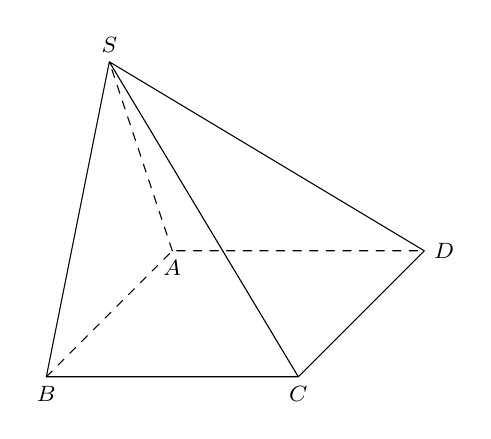
\begin{tikzpicture}[scale=0.8, font=\footnotesize, line join=round, line cap=round, >=stealth]
		\coordinate (a) at (2,2);
		\coordinate (b) at (0,0);
		\coordinate (c) at (4,0);
		\coordinate (d) at (6,2);
		\coordinate (s) at (1,5);
		\draw[dashed] (b) -- (a) -- (d) (a) -- (s);
		\draw (s) -- (b) -- (c) -- (d)-- (s) -- (c);
		\draw (2,2) node[below]{$A$};
		\draw (0,0) node[below]{$B$};
		\draw (4,0) node[below]{$C$};
		\draw (6,2) node[right]{$D$};
		\draw (1,5) node[above]{$S$};
	\end{tikzpicture}	
	}}
\end{ex}

%%%==============Cau_2============%%%
\begin{ex}%[1H8N1-3]
	Cho hình lập phương $ABCD.A_1B_1C_1D_1$. Góc giữa $AC$ và $DA_1$ là
	\choice
	{$90^{\circ}$}                   
	{\True $60^{\circ}$}  
	{$45^{\circ}$}  
	{$120^{\circ}$}  
	\loigiai{
	\immini{
	Vì $A_1C_1 \parallel AC$ nên góc giữa $AC$ và $DA_1$ bằng góc giữa $A_1C_1$ và $DA_1$. \\
	Do tam giác $DA_1C_1$ đều nên $\widehat{DA_1C_1}=60^{\circ}$.\\
	Vậy góc giữa $AC$ và $DA_1$ bằng $60^{\circ}$.	
	}{
	\begin{tikzpicture}[scale=0.6, font=\footnotesize, line join=round, line cap=round, >=stealth]
		\coordinate (a) at (2,2);
		\coordinate (b) at (0,0);
		\coordinate (c) at (5,0);
		\coordinate (d) at (7,2);
		\coordinate (a1) at ($(a)+(0,5)$);
		\coordinate (b1) at ($(b)+(0,5)$);
		\coordinate (c1) at ($(c)+(0,5)$);
		\coordinate (d1) at ($(d)+(0,5)$);
		\draw[dashed] (b) -- (a) -- (d) (a) -- (a1);
		\draw (b) -- (c) -- (d) -- (d1) -- (c1) -- (b1) -- (a1) -- (d1) (b) -- (b1) (c) -- (c1);
		\draw (a) node[below]{$A$};
		\draw (b) node[below]{$B$};
		\draw (c) node[below]{$C$};
		\draw (d) node[right]{$D$};
		\draw (a1) node[above]{$A_1$};
		\draw (b1) node[below left]{$B_1$};
		\draw (c1) node[below right]{$C_1$};
		\draw (d1) node[right]{$D_1$};
		\draw[dashed] (a)-- (c) (d) -- (a1);
		\draw (a1) -- (c1);
	\end{tikzpicture}	
	}
	}
\end{ex}

%%%==============Cau_3============%%%
\begin{ex}%[1H8N1-1]
	Chọn khẳng định đúng trong các khẳng định sau:
	\choice
	{\True Trong không gian, hai đường thẳng vuông góc với nhau có thể cắt nhau hoặc chéo nhau}                   
	{Trong không gian, hai đường thẳng vuông góc với nhau thì phải cắt nhau}  
	{Trong không gian, hai đường thẳng không có điểm chung thì song song với nhau}  
	{Trong không gian, hai đường thẳng phân biệt cùng vuông góc với một đường thẳng thì song song với nhau}  
	\loigiai{
	\immini{
	Giả sử cho hình lập phương $ABCD.A_1B_1C_1D_1$.
	\begin{itemchoice}
		\itemch Đúng, ví dụ $(AB,A_1D_1)=(AB, AD)=90^\circ$.
		\itemch Sai, ví dụ $AA_1\perp DC$ nhưng $AA_1$ và $DC$ ở vị trí chéo nhau.
		\itemch Sai do hai đường thẳng không có điểm chung thì song song hoặc chéo nhau.
		\itemch Sai, ví dụ $AD$ và $CC'$ cùng vuông góc với $CD$ nhưng $AD$ không song song với $CC'$.
	\end{itemchoice}	
	}{
	\begin{tikzpicture}[scale=0.6, font=\footnotesize, line join=round, line cap=round, >=stealth]
		\coordinate (a) at (2,2);
		\coordinate (b) at (0,0);
		\coordinate (c) at (5,0);
		\coordinate (d) at (7,2);
		\coordinate (a1) at ($(a)+(0,5)$);
		\coordinate (b1) at ($(b)+(0,5)$);
		\coordinate (c1) at ($(c)+(0,5)$);
		\coordinate (d1) at ($(d)+(0,5)$);
		\draw[dashed] (b) -- (a) -- (d) (a) -- (a1);
		\draw (b) -- (c) -- (d) -- (d1) -- (c1) -- (b1) -- (a1) -- (d1) (b) -- (b1) (c) -- (c1);
		\draw (a) node[below]{$A$};
		\draw (b) node[below]{$B$};
		\draw (c) node[below]{$C$};
		\draw (d) node[right]{$D$};
		\draw (a1) node[above]{$A_1$};
		\draw (b1) node[below left]{$B_1$};
		\draw (c1) node[below right]{$C_1$};
		\draw (d1) node[right]{$D_1$};
	\end{tikzpicture}	
	}	
	}
\end{ex}


%%%==============Câu_4============%%%
\begin{ex}%[1H8N1-3]
	Cho hình lập phương $ABCD.A'B'C'D'$. Số đo góc tạo bởi hai đường thẳng $BD$ và $AB'$ bằng
	\choice
	{$90^{\circ}$}                   
	{\True $60^{\circ}$}  
	{$45^{\circ}$}  
	{$30^{\circ}$}  
	\loigiai{
	\immini{
	Ta có $AB'\parallel DC' \Leftrightarrow (BD,AB')=(BD,DC')$. \\
	Tam giác $BDC'$ đều vì $BD=BC'=DC'$ (các đường chéo hình vuông bằng nhau) nên $\widehat{BDC'}=60^{\circ}$. \\
	Vậy góc tạo bởi hai đường thẳng $BD$ và $AB'$ bằng $60^{\circ}$.	
	}{
	\begin{tikzpicture}[scale=0.6, font=\footnotesize, line join=round, line cap=round, >=stealth]
		\coordinate (a) at (2,2);
		\coordinate (b) at (0,0);
		\coordinate (c) at (5,0);
		\coordinate (d) at (7,2);
		\coordinate (a1) at ($(a)+(0,5)$);
		\coordinate (b1) at ($(b)+(0,5)$);
		\coordinate (c1) at ($(c)+(0,5)$);
		\coordinate (d1) at ($(d)+(0,5)$);
		\draw[dashed] (b) -- (a) -- (d) (a) -- (a1);
		\draw (b) -- (c) -- (d) -- (d1) -- (c1) -- (b1) -- (a1) -- (d1) (b) -- (b1) (c) -- (c1);
		\draw (a) node[below]{$A$};
		\draw (b) node[below]{$B$};
		\draw (c) node[below]{$C$};
		\draw (d) node[right]{$D$};
		\draw (a1) node[above]{$A'$};
		\draw (b1) node[below left]{$B'$};
		\draw (c1) node[below right]{$C'$};
		\draw (d1) node[right]{$D'$};
		\draw[dashed] (b)-- (d) (b1) -- (a) -- (d1);
		\draw (b1) -- (d1);
	\end{tikzpicture}	
	}
	}
\end{ex}

%%%==============Câu_5============%%%
\begin{ex}%[1H8H1-3]
	Cho tứ diện $ABCD$ có $AB = CD = 2a$. Gọi $M$, $N$ lần lượt là trung điểm của $AD$ và $BC$. Biết $MN = \sqrt{3}a$, góc giữa hai đường thẳng $AB$ và $CD$ bằng
	\choice
	{$45^{\circ}$}
	{$90^{\circ}$}
	{\True $60^{\circ}$}
	{$30^{\circ}$}
	\loigiai{
		\immini
		{
			Gọi $P$ là trung điểm của $AC$.\\
			Khi đó, ta có\\
			$PM\parallel CD$, $PN\parallel AB$.\\
			Suy ra góc giữa $AB$ và $CD$ bằng góc giữa $PM$ và $PN$.\\
			Ta có $PM=\dfrac{CD}{2}=\dfrac{a}{2},PN=\dfrac{AB}{2}=\dfrac{a}{2}$.\\
			Xét tam giác $PMN$ có
			\begin{eqnarray*}
				& \cos\widehat{MPN} & =\dfrac{PM^2+PN^2-MN^2}{2\cdot PM\cdot PN}\\
				& & =\dfrac{\dfrac{a^2}{4}+\dfrac{a^2}{4}-\dfrac{3a^2}{4}}{2\cdot\dfrac{a}{2}\cdot\dfrac{a}{2}}\\
				& & =-\dfrac{1}{2}.	
			\end{eqnarray*}
			Suy ra $\widehat{MPN}=120^{\circ}$.\\
			Suy ra $(PM,PN)=180^{\circ}-120^{\circ}=60^{\circ}$. \\
			Vậy góc giữa hai đường thẳng $AB$ và $CD$ bằng $60^{\circ}$.
		}{
			\begin{tikzpicture}[>=stealth]%Hình 3.4
				\tkzDefPoint(0,0){B}
				\tkzDefShiftPoint[B](0:5){D}
				\tkzDefShiftPoint[B](-60:2){C}
				\tkzDefShiftPoint[B](60:4){A}
				\tkzDefMidPoint(A,D) \tkzGetPoint{M}
				\tkzDefMidPoint(B,C) \tkzGetPoint{N}
				\tkzDefMidPoint(A,C) \tkzGetPoint{P}
				\tkzDrawSegments(A,B A,C A,D B,C C,D N,P M,P)
				\tkzDrawSegments[dashed](B,D M,N)
				\tkzLabelPoint[above](A){\footnotesize $A$}
				\tkzLabelPoint[left](B){\footnotesize $B$}
				\tkzLabelPoint[left](C){\footnotesize $C$}
				\tkzLabelPoint[right](D){\footnotesize $D$}
				\tkzLabelPoint[right](M){\footnotesize $M$}
				\tkzLabelPoint[left](N){\footnotesize $N$}
				\tkzLabelPoint[left](P){\footnotesize $P$}
				\tkzDrawPoints[fill=black](A,B,C,D,M,N,P)
			\end{tikzpicture}
	}
	}
\end{ex}

%%%==============Câu_6============%%%
\begin{ex}%[1H8H1-3]
	Cho hình chóp $SABCD$ có tất cả các cạnh đều bằng $a$ và $O$ là tâm hình vuông $ABCD$. Gọi $M$ là trung điểm $AB$, $N$ là trung điểm $SB$. Gọi $\alpha$ là góc giữa hai đường thẳng $MN$ và $MO$. Khi đó $\cos \alpha$ bằng
	\choice
	{$\dfrac{\sqrt{3}}{2}$}                   
	{\True $\dfrac{1}{2}$}  
	{$\dfrac{\sqrt{2}}{2}$}  
	{$\dfrac{\sqrt{3}}{6}$}  
	\loigiai{
	\immini{
	Ta có hình chóp đều có tất cả các cạnh đều bằng $a$ suy ra tam giác $SAD$ đều và $(SA,AD)=60^{\circ}$. \\
	Mặt khác do $SA\parallel MN$ và $AD \parallel MO$ nên $\alpha=(MN,MO)=(SA,AD)=60^{\circ}$ $\Rightarrow \cos \alpha =\dfrac{1}{2}$.	
	}{
	\begin{tikzpicture}[scale=0.8, font=\footnotesize, line join=round, line cap=round, >=stealth]
		\coordinate (a) at (2,2);
		\coordinate (b) at (0,0);
		\coordinate (c) at (4,0);
		\coordinate (d) at (6,2);
		\coordinate (o) at ($(a)!0.5!(c)$);
		\coordinate (s) at ($(o)+(0,5)$);
		\coordinate (m) at ($(a)!0.5!(b)$);
		\coordinate (n) at ($(s)!0.5!(b)$);
		\draw[dashed] (b) -- (a) -- (d) (c) -- (a) -- (s) (b) -- (d) (n)--(m)--(o);
		\draw (s) -- (b) -- (c) -- (d)-- (s) -- (c);
		\draw (a) node[below]{$A$};
		\draw (b) node[below]{$B$};
		\draw (c) node[below]{$C$};
		\draw (d) node[right]{$D$};
		\draw (s) node[above]{$S$};
		\draw (o) node[above]{$O$};
		\draw (m) node[left]{$M$};
		\draw (n) node[above left]{$N$};
	\end{tikzpicture}	
	}
	}
\end{ex}

%%%==============Câu_7============%%%
\begin{ex}%[1H8H1-3]
	Cho hình lập phương $ABCD.A'B'C'D'$ cạnh $a$, $M$ là trung điểm $CD$. Gọi $\alpha$ là góc tạo bởi $A'B$ và $D'M$. Tính $\cos \alpha$.
	\choice
	{$\cos \alpha=\dfrac{1}{2}$}                   
	{\True $\cos \alpha=\dfrac{3\sqrt{5}}{5}$}  
	{$\cos \alpha=\dfrac{\sqrt{2}}{2}$}  
	{$\cos \alpha=\dfrac{\sqrt{10}}{10}$}  
	\loigiai{
	\immini{
	Ta có $D'C\parallel A'B$ nên $(A'B,D'M)=(D'C,D'M)=\alpha$. \\
	Có $D'M=\dfrac{a\sqrt{5}}{2}$, $D'C=a\sqrt{2}$, $CM=\dfrac{a}{2}$. \\
	Tam giác $D'MC$ có $$\cos \alpha=\dfrac{D'M^2+D'C^2-CM^2}{2D'M.D'C}=\dfrac{3\sqrt{5}}{5}.$$	
	}{
	\begin{tikzpicture}[scale=0.6, font=\footnotesize, line join=round, line cap=round, >=stealth]
		\coordinate (a) at (2,2);
		\coordinate (b) at (0,0);
		\coordinate (c) at (5,0);
		\coordinate (d) at (7,2);
		\coordinate (a1) at ($(a)+(0,5)$);
		\coordinate (b1) at ($(b)+(0,5)$);
		\coordinate (c1) at ($(c)+(0,5)$);
		\coordinate (d1) at ($(d)+(0,5)$);
		\coordinate (m) at ($(c)!0.5!(d)$);
		\draw[dashed] (b) -- (a) -- (d) (a) -- (a1);
		\draw (b) -- (c) -- (d) -- (d1) -- (c1) -- (b1) -- (a1) -- (d1) (b) -- (b1) (c) -- (c1);
		\draw (a) node[below]{$A$};
		\draw (b) node[below]{$B$};
		\draw (c) node[below]{$C$};
		\draw (d) node[right]{$D$};
		\draw (a1) node[above]{$A'$};
		\draw (b1) node[below left]{$B'$};
		\draw (c1) node[below right]{$C'$};
		\draw (d1) node[right]{$D'$};
		\draw (m) node[right]{$M$};
		\draw[dashed] (a1)-- (b);
		\draw (m) -- (d1) -- (c);
	\end{tikzpicture}	
	}
	}
\end{ex}

%%%==============Câu_8============%%%
\begin{ex}%[1H8H1-3]
	Cho hình chóp $SABCD$ có tất cả các cạnh đều bằng $a$. Gọi $I$ và $J$ lần lượt là trung điểm của $SC$ và $BC$. Số đo góc $(IJ,CD)$ bằng 
	\choice
	{\True $60^{\circ}$}
	{$45^{\circ}$}
	{$30^{\circ}$}
	{$90^{\circ}$}
	\loigiai{
	\immini{
	Gọi $O$ là tâm của hình vuông $ABCD$, ta có $OJ \parallel CD$.\\ $\Rightarrow (IJ,CD)=(IJ,OJ)$. \\
	Tam giác $OIJ$ có $IJ=OJ=OI=\dfrac{SB}{2}=\dfrac{a}{2}$ nên tam giác $OIJ$ đều. \\
	Vậy $(IJ,CD)=(IJ,OJ)=60^{\circ}$.	
	}{
	\begin{tikzpicture}[scale=0.7, font=\footnotesize, line join=round, line cap=round, >=stealth]
		\coordinate (a) at (2,2);
		\coordinate (b) at (0,0);
		\coordinate (c) at (4,0);
		\coordinate (d) at (6,2);
		\coordinate (o) at ($(a)!0.5!(c)$);
		\coordinate (s) at ($(o)+(0,5)$);
		\coordinate (i) at ($(s)!0.5!(c)$);
		\coordinate (j) at ($(c)!0.5!(b)$);
		\draw[dashed] (b) -- (a) -- (d) (c) -- (a) -- (s) (b) -- (d);
		\draw (s) -- (b) -- (c) -- (d)-- (s) -- (c);
		\draw (a) node[below]{$A$};
		\draw (b) node[below]{$B$};
		\draw (c) node[below]{$C$};
		\draw (d) node[right]{$D$};
		\draw (s) node[above]{$S$};
		\draw (o) node[above]{$O$};
		\draw (i) node[left]{$I$};
		\draw (j) node[below]{$J$};
		\draw (i) -- (j);
		\draw[dashed] (i)--(o) -- (j);
	\end{tikzpicture}	
	}		
	}
\end{ex}

%%%==============Câu_9============%%%
\begin{ex}%[1H8H1-3]
	Cho tứ diện $ABCD$ có tất cả các cạnh bằng $a$. Gọi $M$ là trung điểm $BC$ và $N$ là trung điểm $AB$. Gọi $\alpha$ là góc giữa hai đường thẳng $DM$ và $MN$
	\choice
	{$\dfrac{\sqrt{3}}{2}$}                   
	{$\dfrac{1}{2}$}  
	{$\dfrac{\sqrt{2}}{2}$}  
	{\True $\dfrac{\sqrt{3}}{6}$}  
	\loigiai{
	\immini{
	Có $MN=\dfrac{AC}{2}=\dfrac{a}{2}$. \\
	$\cos DMN=\dfrac{DM^2+MN^2-ND^2}{2DM.MN}=\dfrac{\sqrt{3}}{6}$. \\
	Suy ra $\cos \alpha=\cos (DM,MN)=\dfrac{\sqrt{3}}{6}$.	
	}{
	\begin{tikzpicture}[scale=0.7, font=\footnotesize, line join=round, line cap=round, >=stealth]
		\coordinate (a) at (2,2);
		\coordinate (b) at (0,0);
		\coordinate (c) at (4,0);
		\coordinate (d) at (6,2);
		\coordinate (o) at ($(a)!0.5!(c)$);
		\coordinate (s) at ($(o)+(0,5)$);
		\coordinate (m) at ($(b)!0.5!(c)$);
		\coordinate (n) at ($(a)!0.5!(b)$);
		\draw[dashed] (b) -- (a) -- (d) (c) -- (a) -- (s) (b) -- (d);
		\draw (s) -- (b) -- (c) -- (d)-- (s) -- (c);
		\draw (a) node[below]{$A$};
		\draw (b) node[below]{$B$};
		\draw (c) node[below]{$C$};
		\draw (d) node[right]{$D$};
		\draw (s) node[above]{$S$};
		\draw (o) node[above]{$O$};
		\draw (m) node[below]{$M$};
		\draw (n) node[right]{$N$};
		\draw[dashed] (d)--(m) -- (n);
	\end{tikzpicture}	
	}		
	}
\end{ex}

%%%==============Câu_10============%%%
\begin{ex}%[1H8N1-3]
	Cho hình chóp $SABCD$ có đáy là hình vuông $ABCD$ cạnh $a$ và các cạnh bên bằng $a$. Gọi $M$, $N$ lần lượt là trung điểm $AD$ và $SD$. Số đo góc $(MN,SC)$ bằng 
	\choice
	{$60^{\circ}$}
	{$45^{\circ}$}
	{$30^{\circ}$}
	{\True $90^{\circ}$}
	\loigiai{
	\immini{
	Tam giác $SAC$ có $SA=SC=a$ và $AC=a\sqrt{2}$ nên tam giác $SAC$ vuông cân tại $S$. \\
	Ta có $MN\parallel SA$ nên $(MN,SC)=(SA,SC)=90^{\circ}$.	
	}{
	\begin{tikzpicture}[scale=0.8, font=\footnotesize, line join=round, line cap=round, >=stealth]
		\coordinate (a) at (2,2);
		\coordinate (b) at (0,0);
		\coordinate (c) at (4,0);
		\coordinate (d) at (6,2);
		\coordinate (o) at ($(a)!0.5!(c)$);
		\coordinate (s) at ($(o)+(0,5)$);
		\coordinate (m) at ($(a)!0.5!(d)$);
		\coordinate (n) at ($(s)!0.5!(d)$);
		\draw[dashed] (b) -- (a) -- (d) (c) -- (a) -- (s) (b) -- (d);
		\draw (s) -- (b) -- (c) -- (d)-- (s) -- (c);
		\draw (a) node[below]{$A$};
		\draw (b) node[below]{$B$};
		\draw (c) node[below]{$C$};
		\draw (d) node[right]{$D$};
		\draw (s) node[above]{$S$};
		\draw (o) node[above]{$O$};
		\draw (m) node[below]{$M$};
		\draw (n) node[right]{$N$};
		\draw[dashed] (d)--(m) -- (n);
	\end{tikzpicture}}}
\end{ex}

%%%==============Câu_11============%%%
\begin{ex}%[1H8V1-2]
	Cho hình lập phương $ABCD.A'B'C'D'$. Trong số $5$ đường thẳng $AC'$, $AB'$, $BD$, $C'D$, $BC'$ có bao nhiêu đường thẳng vuông góc với $A'C$?
	\choice
	{$1$}                   
	{$2$}  
	{$3$}  
	{\True $4$}  
	\loigiai{
	\immini{
	Ta có $A'C \perp (BDC')$ vì $A'$ và $C$ cách đều ba đỉnh $B,D,C'$.\\
	Như vậy đường nào song song hoặc nằm trong mặt phẳng $(BDC')$ đều vuông góc với $A'C$.\\
	Có 4 đường thỏa là $AB'$, $BD$, $C'D$, $BC'$.	
	}{
	\begin{tikzpicture}[scale=0.6, font=\footnotesize, line join=round, line cap=round, >=stealth]
		\coordinate (a) at (1,2);
		\coordinate (b) at (0,0);
		\coordinate (c) at (5,0);
		\coordinate (d) at (6,2);
		\coordinate (a1) at ($(a)+(0,5)$);
		\coordinate (b1) at ($(b)+(0,5)$);
		\coordinate (c1) at ($(c)+(0,5)$);
		\coordinate (d1) at ($(d)+(0,5)$);
		\coordinate (m) at ($(c)!0.5!(d)$);
		\draw[dashed] (b) -- (a) -- (d) (a) -- (a1);
		\draw (b) -- (c) -- (d) -- (d1) -- (c1) -- (b1) -- (a1) -- (d1) (b) -- (b1) (c) -- (c1);
		\draw (a) node[below]{$A$};
		\draw (b) node[below]{$B$};
		\draw (c) node[below]{$C$};
		\draw (d) node[right]{$D$};
		\draw (a1) node[above]{$A'$};
		\draw (b1) node[below left]{$B'$};
		\draw (c1) node[below right]{$C'$};
		\draw (d1) node[right]{$D'$};
		\draw (m) node[right]{$M$};
		\draw[dashed] (a)-- (c1) (a) -- (b1) (b) -- (d) (a1) --(c);
		\draw (c1) -- (d) (b)--(c1);
	\end{tikzpicture}	
	}
	}
\end{ex}

%%%==============Câu_12============%%%
\begin{ex}%[1H8V1-3]
	Cho hình lập phương $ABCD.A'B'C'D'$. Gọi $M$, $N$, $P$ lần lượt là trung điểm các cạnh $AB$, $BC$, $C'D'$. Tính góc giữa hai đường thẳng $MN$ và $AP$.
	\choice
	{$30^{\circ}$}
	{$60^{\circ}$}
	{$135^{\circ}$}
	{\True $45^{\circ}$}
	\loigiai{
	\immini{
	Tam giác $A'D'P$ vuông tại $D'$, ta có $$A'P=\sqrt{A'D'^2+D'P^2}=\dfrac{a\sqrt{5}}{2}.$$
	Tam giác $AA'P$ vuông tại $A'$, ta có
	$$AP=\sqrt{A'A^2+A'P^2}=\dfrac{3a}{2}.$$
	Tam giác $CC'P$ vuông tại $C'$, ta có $$CP=\sqrt{C'C^2+C'P^2}=\dfrac{a\sqrt{5}}{2}.$$
	$AC$ là đường chéo hình vuông cạnh $a$ nên $AC=a\sqrt{2}$. \\
	Tam giác $ACP$ có
		$$CP^2=AC^2+AP^2-2AC.AP.\cos CAP$$
		$$\Rightarrow \cos CAP=\dfrac{1}{2}
		\Rightarrow \widehat{CAP}=45^{\circ}$$
	Vậy $(MN,AP)=\widehat{CAP}=45^{\circ}$.	
	}{
		\begin{tikzpicture}[scale=0.6, font=\footnotesize, line join=round, line cap=round, >=stealth]
		\coordinate (a) at (2,2);
		\coordinate (b) at (0,0);
		\coordinate (c) at (5,0);
		\coordinate (d) at (7,2);
		\coordinate (a1) at ($(a)+(0,5)$);
		\coordinate (b1) at ($(b)+(0,5)$);
		\coordinate (c1) at ($(c)+(0,5)$);
		\coordinate (d1) at ($(d)+(0,5)$);
		\coordinate (m) at ($(a)!0.5!(b)$);
		\coordinate (n) at ($(b)!0.5!(c)$);
		\coordinate (p) at ($(c1)!0.5!(d1)$);
		\draw[dashed] (b) -- (a) -- (d) (a) -- (a1);
		\draw (b) -- (c) -- (d) -- (d1) -- (c1) -- (b1) -- (a1) -- (d1) (b) -- (b1) (c) -- (c1);
		\draw (a) node[below]{$A$};
		\draw (b) node[below]{$B$};
		\draw (c) node[below]{$C$};
		\draw (d) node[right]{$D$};
		\draw (a1) node[above]{$A'$};
		\draw (b1) node[below left]{$B'$};
		\draw (c1) node[below right]{$C'$};
		\draw (d1) node[right]{$D'$};
		\draw (m) node[left]{$M$};
		\draw (n) node[below]{$N$};
		\draw (p) node[below]{$P$};
		\draw[dashed] (m)-- (n) (a)--(p) (a)--(c);
	\end{tikzpicture}	
	}	
	}
\end{ex}


\Closesolutionfile{ans}
\indapan{6}{ans/ans-1-C8B1.De2}
\cauds 
\Opensolutionfile{ans}[ans/ans-1-C8B1.De2-DS]
%%%==============Câu_1============%%%
\begin{ex}%[1H8V1-2]
	Cho tứ diện $ABCD$ có $AB=AC=AD=1$, $\widehat{BAC}=\widehat{BAD}=60^{\circ}$ và $\widehat{CAD}=90^{\circ}$. Gọi $I$, $J$ lần lượt là trung điểm $AB$ và $CD$. Xét tính đúng sai của các khẳng định sau:
	\choiceTF
	{\True $CD=\sqrt{2}$}
	{Tam giác $BCD$ vuông cân tại $C$}
	{\True $IJ\perp AB$}
	{\True $IJ\perp CD$}
	\loigiai{
			\begin{center}
			\begin{tikzpicture}[scale=0.8, font=\footnotesize, line join=round, line cap=round, >=stealth]
				\coordinate (a) at (3,4);
				\coordinate (b) at (0,0);
				\coordinate (c) at (2,-2);
				\coordinate (d) at (5,0);
				\coordinate (i) at ($(a)!0.5!(b)$);
				\coordinate (j) at ($(c)!0.5!(d)$);
				\draw[dashed] (b) -- (d);
				\draw (a) -- (b) -- (c) -- (d) -- (a) -- (c);
				\draw (a) node[above]{$A$};
				\draw (b) node[left]{$B$};
				\draw (c) node[below]{$C$};
				\draw (d) node[right]{$D$};
				\draw (i) node[left]{$I$};
				\draw (j) node[below]{$J$};
				\draw[dashed] (i)-- (j) (i)--(d);
				\draw (i) -- (c);
			\end{tikzpicture}
		\end{center}
		Các tam giác $ABC$ và $ABD$ cân tại $A$ và có góc $60^{\circ}$ nên hai tam giác $ABC$ và $ABD$ là tam giác đều cạnh bằng $1$.
		\begin{itemchoice}
			\itemch Đúng. Vì tam giác $ACD$ vuông cân tại $A$ nên $CD=\sqrt{1^2+1^2}=\sqrt{2}$.
			\itemch Sai.\\ 
				Tam giác $BCD$ có $BC^2=1,BD^2=1,CD^2=2$.\\
				Suy ra $BC^2+BD^2=CD^2$. \\
				Vậy tam giác $BCD$ vuông cân tại $B$.
			\itemch Đúng.\\ 
				Ta có $AJ=BJ=\dfrac{\sqrt{2}}{2}$ nên tam giác $JAB$ cân tại $J$.\\
				Mặt khác $I$ là trung điểm $AB$ nên $IJ \perp AB$.
			\itemch Đúng.\\ 
				Tam giác $ABC$ và $A B D$ đều cạnh 1 nên $CI=DI=\dfrac{\sqrt{3}}{2}$. 
				Vì vậy tam giác $I C D$ cân tại $I$, mà $J$ là trung điểm $CD$ nên $IJ \perp CD$.
	\end{itemchoice}}
\end{ex}

%%%==============Câu_2============%%%
\begin{ex}%[1H8V1-2]
	Cho hình hộp $ABCD.A'B'C'D'$ có tất cả các cạnh bằng nhau. Xét tính đúng sai của các khẳng định sau: 
	\choiceTF
	{ $ABCD$ là hình chữ nhật}
	{\True $A'C'\perp BD$}
	{\True $A'B\perp DC'$}
	{\True $BC'\perp A'D$}
	\loigiai{
		\begin{center}
			\begin{tikzpicture}[scale=0.6, font=\footnotesize, line join=round, line cap=round, >=stealth]
				\coordinate (a) at (2,2);
				\coordinate (b) at (0,0);
				\coordinate (c) at (5,0);
				\coordinate (d) at (7,2);
				\coordinate (a1) at ($(a)+(1,5)$);
				\coordinate (b1) at ($(b)+(1,5)$);
				\coordinate (c1) at ($(c)+(1,5)$);
				\coordinate (d1) at ($(d)+(1,5)$);
				\draw[dashed] (b) -- (a) -- (d) (a) -- (a1);
				\draw (b) -- (c) -- (d) -- (d1) -- (c1) -- (b1) -- (a1) -- (d1) (b) -- (b1) (c) -- (c1);
				\draw (a) node[below]{$A$};
				\draw (b) node[below]{$B$};
				\draw (c) node[below]{$C$};
				\draw (d) node[right]{$D$};
				\draw (a1) node[above]{$A'$};
				\draw (b1) node[below left]{$B'$};
				\draw (c1) node[below right]{$C'$};
				\draw (d1) node[right]{$D'$};
				\draw (a1)--(c1) (d)--(c1);
				\draw[dashed] (b)--(d) (a1)--(b);
			\end{tikzpicture}
		\end{center}
		Vì hình hộp $ABCD.A'B'C'D'$ có tất cả các cạnh đều bằng nhau nên các tứ giác $ABCD$, $A'B'BA$, $B'C'CB$ đều là hình thoi.
		\begin{itemchoice}
			\itemch Sai vì $ABCD$ là hình bình hành.
			\itemch Sai. Vì $AC\perp BD$ mà $AC \parallel A'C'$ nên $A'C'\perp BD$.
			\itemch Đúng. Vì $A'B\perp AB'$ mà $AB' \parallel DC'$ nên $A'B\perp DC'$.
			\itemch Đúng. Vì $BC'\perp B'C$ mà $B'C \parallel A'D$ nên $BC'\perp A'D$.
	\end{itemchoice}}
\end{ex}

%%%==============Câu_3============%%%
\begin{ex}%[1H8V1-3]
	Cho hình hộp $ABCD.A'B'C'D'$ có 6 mặt là hình vuông cạnh $a$. Xét tính đúng sai của các khẳng định sau: 
	\choiceTF
	{\True $BC' \parallel AD'$}
	{\True $(AD',B'C)=90^{\circ}$}
	{\True $(AD',DC')=(BC',DC')$}
	{$\widehat{BC'D}=90^{\circ}$}
	\loigiai{	
		\begin{center}
			\begin{tikzpicture}[scale=0.7, font=\footnotesize, line join=round, line cap=round, >=stealth]
				\coordinate (a) at (1,2);
				\coordinate (b) at (0,0);
				\coordinate (c) at (5,0);
				\coordinate (d) at (6,2);
				\coordinate (a1) at ($(a)+(0,5)$);
				\coordinate (b1) at ($(b)+(0,5)$);
				\coordinate (c1) at ($(c)+(0,5)$);
				\coordinate (d1) at ($(d)+(0,5)$);
				\draw[dashed] (b) -- (a) -- (d) (a) -- (a1);
				\draw (b) -- (c) -- (d) -- (d1) -- (c1) -- (b1) -- (a1) -- (d1) (b) -- (b1) (c) -- (c1);
				\draw (a) node[below]{$A$};
				\draw (b) node[below]{$B$};
				\draw (c) node[below]{$C$};
				\draw (d) node[right]{$D$};
				\draw (a1) node[above]{$A'$};
				\draw (b1) node[below left]{$B'$};
				\draw (c1) node[below right]{$C'$};
				\draw (d1) node[right]{$D'$};
				\draw (b) -- (c1)--(d);
			\end{tikzpicture}
		\end{center}
		\begin{itemchoice}
			\itemch Đúng. Vì $ABCD.A'B'C'D'$ là hình hộp nên $AB=C'D'$ và $AB \parallel C'D'$ nên $ABX'D'$ là hình bình hành.\\
			Vậy $BC' \parallel AD'$.
			\itemch Đúng. Vì $BC'\parallel AD'$ nên $(AD',B'C)=90^{\circ}$.
			\itemch Đúng. Vì $BC'\parallel AD'$ nên $(AD',DC')=(BC',DC')$.
			\itemch Sai. Vì tam giác $BC'D$ đều nên $\widehat{BC'D}=60^{\circ}$.
	\end{itemchoice}}
\end{ex}

%%%==============Câu_4============%%%
\begin{ex}%[1H8V1-3]
	Cho hình lăng trụ tam giác $ABC.A'B'C'$ có $AA'\perp AB$, $AA'\perp AC$ và tất cả các cạnh đều bằng $a$. Gọi $M$ là trung điểm $AA'$. Xét tính đúng sai của các khẳng định sau: 
	\choiceTF
	{\True $(A'B,C'C)=\widehat{AA'B}$}
	{\True $(A'B,C'C)=45^{\circ}$}
	{$(A'C,MB)=\widehat{BAC}$}
	{$\widehat{BMN}\approx 42{,}6^{\circ}$}
	\loigiai{		
		\begin{center}
			\begin{tikzpicture}[scale=0.7, font=\footnotesize, line join=round, line cap=round, >=stealth]
				\coordinate (a) at (0,0);
				\coordinate (b) at (2,-2);
				\coordinate (c) at (5,0);
				\coordinate (a1) at ($(a)+(0,5)$);
				\coordinate (b1) at ($(b)+(0,5)$);
				\coordinate (c1) at ($(c)+(0,5)$);
				\coordinate (m) at ($(a)!0.5!(a1)$);
				\draw[dashed] (a) -- (c);
				\draw (a) -- (b) -- (c) -- (c1) -- (b1) -- (b) (a) -- (a1)--(b1) (a1)-- (c1);
				\draw (a) node[below]{$A$};
				\draw (b) node[below]{$B$};
				\draw (c) node[below]{$C$};
				\draw (a1) node[above]{$A'$};
				\draw (b1) node[below left]{$B'$};
				\draw (c1) node[below right]{$C'$};
				\draw (m) node[left]{$M$};
				\draw (a1) -- (b) -- (m);
			\end{tikzpicture}
		\end{center}
		\begin{itemchoice}
			\itemch Đúng. Vì $A'A\parallel C'C \Rightarrow (A'B,C'C)=(A'B,A'A)=\widehat{AA'B}$.
			\itemch Đúng. Vì tam giác $A'AB$ vuông cân tại $A$ nên $\widehat{AA'B}=45^\circ$.
			\itemch Sai.\\
				Gọi $N$ là trung điểm $AC$. \\
				Ta có $A'C \parallel MN \Rightarrow (A'C,MB)=(MN,MB)=\widehat{BMN}$.
			\itemch Sai.\\
				Tam giác $MNB$ có $MB=MN=\sqrt{a^2+\dfrac{a^2}{4}}=\dfrac{a\sqrt{5}}{2}$ và $BN=\dfrac{a\sqrt{3}}{2}$. \\
				$\Rightarrow \cos BMN=\dfrac{7}{10} \Rightarrow \widehat{BMN} \approx 45{,}6^\circ$.
	\end{itemchoice}}
\end{ex}


\Closesolutionfile{ans}
\indapan{2}{ans/ans-1-C8B1.De2-DS}
%-------

\Opensolutionfile{ans}[ans/ans-1-C8B1.De2-KQ]
\caukq
%Phan 3
%%%==============Câu_1============%%%
\begin{ex}%[1H8H1-3]
	Cho tứ diện đều $ABCD$. Gọi $M$ là trung điểm của cạnh $BC$. Côsin của góc giữa hai đường thẳng $A B$ và $D M$ bằng $\dfrac{\sqrt{a}}{6}$. Giá trị của $a$ là
	\shortans{$3$}
	\loigiai{
	\immini{
	Kẻ $M N \parallel A B$, có $M N$ là đường trung bình của $\triangle ABC$.
	Suy ra $M N=\dfrac{AB}{2}$. \\
	Do đó $(AB, DM)=(MN, DM)=\widehat{DMN}=\alpha$. \\
	Gọi tứ diện đều $A B C D$ có cạnh bằng $a$. \\
	$MN=\dfrac{a}{2}, DN=DM=\dfrac{a\sqrt{3}}{2}$ \\
	$\Rightarrow \cos \alpha=\dfrac{MN^2+DM^2-DN^2}{2\cdot MN\cdot DM}=\dfrac{\sqrt{3}}{6}$.	
	}{
	\begin{tikzpicture}[scale=0.7, font=\footnotesize, line join=round, line cap=round, >=stealth]
		\coordinate (b) at (0,0);
		\coordinate (c) at (2,-2);
		\coordinate (d) at (5,0);
		\coordinate (m) at ($(b)!0.5!(c)$);
		\coordinate (p) at ($(c)!0.5!(d)$);	
		\draw[dashed, name path=dm](d)--(m);
		\draw[dashed, name path=bp] (b)--(p);
		\path [name intersections={of=dm and bp,by=o}];
		\coordinate (a) at ($(o)+(0,5)$);
		\coordinate (n) at ($(a)!0.5!(c)$);
		\draw (o) node[above right]{O};
		
		\draw[dashed] (b) -- (d);
		\draw (a) -- (b) -- (c) -- (d) -- (a) -- (c) (m)--(n) -- (d);
		\draw (a) node[above]{$A$};
		\draw (b) node[below left]{$B$};
		\draw (c) node[below]{$C$};
		\draw (d) node[below right]{$D$};
		\draw (n) node[left]{$N$};
		\draw (m) node[left]{$M$};
	\end{tikzpicture}	
	}}
\end{ex}

%%%==============Câu_2============%%%
\begin{ex}%[1H8H1-3]
	Cho hình lăng trụ đứng $ABC.A'B'C'$ có $AB=AC=a$, $\widehat{BAC}=120^\circ$, $AA'=a\sqrt{2}$. Góc giữa hai đường thẳng $AB'$ và $BC$ bằng $a^\circ$. Giá trị của $a$ là
	\shortans{$60$}
	\loigiai{
	\immini{
		Ta có: $B'C'=BC=a\sqrt{3}, AB'=\sqrt{AB^2+B'A^2}=a\sqrt{3}$ \\
	$AC'=\sqrt{C'A^2+AC^2}=a\sqrt{3}$. \\
	Vậy tam giác $B'AD$ đều nên $\widehat{B'AD}=60^{\circ}$. \\		
	Ta có $BC \parallel B'C'$ nên 
	$$(AB',BC)=(AB',B'C')=\widehat{B'AD}=60^{\circ}.$$ 	
	}{
	\begin{tikzpicture}[scale=0.7, font=\footnotesize, line join=round, line cap=round, >=stealth]
		\coordinate (a) at (0,0);
		\coordinate (b) at (2,-2);
		\coordinate (c) at (5,0);
		\coordinate (a1) at ($(a)+(0,5)$);
		\coordinate (b1) at ($(b)+(0,5)$);
		\coordinate (c1) at ($(c)+(0,5)$);
		\draw[dashed] (a) -- (c);
		\draw (a) -- (b) -- (c) -- (c1) -- (b1) -- (b) (a) -- (a1)--(b1) (a1)-- (c1);
		\draw (a) node[below]{$A$};
		\draw (b) node[below]{$B$};
		\draw (c) node[below]{$C$};
		\draw (a1) node[above]{$A'$};
		\draw (b1) node[below left]{$B'$};
		\draw (c1) node[below right]{$C'$};
		\draw (a) -- (b1);
	\end{tikzpicture}	
	}
	}
\end{ex}

%%%==============Câu_3============%%%
\begin{ex}%[1H8V1-3]
	Cho hình chóp $S.ABC$ có $SA, SB,SC$ đôi một vuông góc với nhau và $SA=SB=SC=a$. Gọi $M$ là trung điểm của $AB$. Góc giữa hai đường thẳng $SM$ và $BC$ bằng $a^\circ$. Giá trị của $a$ là
	\shortans{$60$}
	\loigiai{
	\immini{
	Gọi $N$ là trung điểm của $AC$. Khi đó góc giữa $SM$ và $BC$ bằng góc giữa $SM$ và $MN$. \\
	Ta có $AB=BC=CA$.\\
	$SM=\dfrac{1}{2} AB$ (trung tuyến trong tam giác vuông ứng với cạnh huyền). \\
	$SN=\dfrac{1}{2} AC$ (trung tuyến trong tam giác vuông ứng với cạnh huyền). \\
	$MN=\dfrac{1}{2} BC$. \\
	Suy ra $SM=MN=SN$ hay tam giác $SMN$ đều. \\
	Do đó $(SM;BC)=\widehat{SMN}=60^{\circ}$.	
	}{
	\begin{tikzpicture}[scale=0.8, font=\footnotesize, line join=round, line cap=round, >=stealth]
		\coordinate (s) at (0,0);
		\coordinate (a) at (0,4);
		\coordinate (b) at (-2,-2);
		\coordinate (c) at (4,0);
		\coordinate (m) at ($(a)!0.5!(b)$);
		\coordinate (n) at ($(a)!0.5!(c)$);
		\draw[dashed] (b) -- (s) -- (c) (s)--(a) (m)--(s)--(n);
		\draw (a) -- (b) -- (c) -- (a) (m)--(n) ;
		\draw (a) node[above]{$A$};
		\draw (b) node[below]{$B$};
		\draw (c) node[below]{$C$};
		\draw (s) node[below]{$S$};
		\draw (m) node[left]{$M$};
		\draw (n) node[right]{$N$};
	\end{tikzpicture}	
	}	
	}
\end{ex}

%%%==============Câu_4============%%%
\begin{ex}%[1H8V1-3]
	Cho hình hộp $ABCD.A'B'C'D'$ có $6$ mặt là hình vuông. Số đo của góc giữa hai đường thẳng $AC$ và $A'D$ bằng $a^\circ$. Giá trị của $a$ là
	\shortans{$60$}
	\loigiai{
	\immini{
	Ta có $(AC,A'D)=(A'C',A'D)=\widehat{DA'C'}=60^{\circ}$.	
	}{
	\begin{tikzpicture}[scale=0.6, font=\footnotesize, line join=round, line cap=round, >=stealth]
		\coordinate (a) at (2,2);
		\coordinate (b) at (0,0);
		\coordinate (c) at (5,0);
		\coordinate (d) at (7,2);
		\coordinate (a1) at ($(a)+(0,5)$);
		\coordinate (b1) at ($(b)+(0,5)$);
		\coordinate (c1) at ($(c)+(0,5)$);
		\coordinate (d1) at ($(d)+(0,5)$);
		\draw[dashed] (b) -- (a) -- (d) (c) -- (a) -- (a1) (a1)--(d);
		\draw (b) -- (c) -- (d) -- (d1) -- (c1) -- (b1) -- (a1) -- (d1) (b) -- (b1) (c) -- (c1) (a1)--(c1);
		\draw (a) node[below]{$A$};
		\draw (b) node[below]{$B$};
		\draw (c) node[below]{$C$};
		\draw (d) node[right]{$D$};
		\draw (a1) node[above]{$A'$};
		\draw (b1) node[below left]{$B'$};
		\draw (c1) node[below right]{$C'$};
		\draw (d1) node[right]{$D'$};
	\end{tikzpicture}	
	}
	}
\end{ex}

%%%==============Câu_5============%%%
\begin{ex}%[1H8C1-3]
	Cho hình hộp $ABCD.A'B'C'D'$ có $6$ mặt là hình vuông cạnh $a$. Gọi $M$, $N$ lần lượt là trung điểm của $AA'$ và $A'B'$. Góc giữa hai đường thẳng $MN$ và $BD$ bằng $a^\circ$. Giá trị của $a$ là
	\shortans{$60$}
	\loigiai{
	\immini{
		Gọi $P$ là trung điểm $A'D'$. Ta có $NP\parallel BD$.\\
	Do $ABCD.A'B'C'D'$ là hình lập phương cạnh $a$ nên $AB'=B'D'=D'A=a\sqrt{2}$. \\
	Suy ra $MN=NP=PM=\dfrac{a\sqrt{2}}{2}$. \\
	Suy ra $(MN,BD)=(MN,NP)=60^\circ$.	
	}{
	\begin{tikzpicture}[scale=0.6, font=\footnotesize, line join=round, line cap=round, >=stealth]
		\coordinate (a) at (2,2);
		\coordinate (b) at (0,0);
		\coordinate (c) at (5,0);
		\coordinate (d) at (7,2);
		\coordinate (a1) at ($(a)+(0,5)$);
		\coordinate (b1) at ($(b)+(0,5)$);
		\coordinate (c1) at ($(c)+(0,5)$);
		\coordinate (d1) at ($(d)+(0,5)$);
		\coordinate (m) at ($(a)!0.5!(a1)$);
		\coordinate (n) at ($(a1)!0.5!(b1)$);
		\coordinate (p) at ($(a1)!0.5!(d1)$);
		\draw[dashed] (b) -- (a) -- (d) --(b) (a) -- (a1) (n)--(m)--(p) ;
		\draw (b) -- (c) -- (d) -- (d1) -- (c1) -- (b1) -- (a1) -- (d1) (b) -- (b1) (c) -- (c1) (n)--(p);
		\draw (a) node[below]{$A$};
		\draw (b) node[below]{$B$};
		\draw (c) node[below]{$C$};
		\draw (d) node[right]{$D$};
		\draw (a1) node[above]{$A'$};
		\draw (b1) node[below left]{$B'$};
		\draw (c1) node[below right]{$C'$};
		\draw (d1) node[right]{$D'$};
		\draw (m) node[below right]{$M$};
		\draw (n) node[left]{$N$};
		\draw (p) node[above]{$P$};
		%				\draw (b) -- (c1)--(d);
	\end{tikzpicture}		
	}
	}
\end{ex}

%%%==============Câu_6============%%%
\begin{ex}%[1H8C1-3]
	Cho hình chóp $S.ABC$ có $SA=SB=SC$, $\widehat{BSC}=\widehat{CSA}=60^{\circ}$, $\widehat{BSA}=90^{\circ}$. Gọi $E,F$ lần lượt là trung điểm của $AB$ và $SC$. Số đo góc của hai đường thẳng $EF$ và $SC$ bằng $a^\circ$. Giá trị của $a$ là
	\shortans{$90$}
	\loigiai{
	\immini{
	Gọi $SA=SB=SC=x$. \\
	Ta có $\triangle SAC$ và $\triangle SBC$ cân và có một góc $60^{\circ}$ nên là hai tam giác đều.\\
	Suy ra $AC=BC=x$.\\
	$\triangle SAB$ vuông cân tại $S$ nên $AB=x\sqrt{2}$.\\
	Xét $\triangle ABC$ có $AC=BC=x$ và $AB=x\sqrt{2}$ nên $\triangle ABC$ vuông cân tại $C$. \\
	Suy ra $CE=SE=\dfrac{AB}{2}$. \\
	$\triangle SCE$ cân tại $E$ có $EF$ là trung tuyến nên là đường cao $\Rightarrow EF \perp SC$.\\
	Vậy $(EF,SC)=90^\circ$.
	}{
	\begin{tikzpicture}[scale=1, font=\footnotesize, line join=round, line cap=round, >=stealth]
		\coordinate (a) at (0,0);
		\coordinate (c) at (2,-2);
		\coordinate (b) at (6,0);
		\coordinate (e) at ($(a)!0.5!(b)$);
		\coordinate (s) at ($(e)+(0,4)$);
		\coordinate (f) at ($(s)!0.5!(c)$);
		\draw[dashed] (a) -- (b) (s) -- (e) -- (c) (e)--(f);
		\draw (s) -- (a) -- (c) -- (b) -- (s) -- (c);
		\draw (a) node[below]{$A$};
		\draw (c) node[below]{$C$};
		\draw (b) node[below]{$B$};
		\draw (s) node[above]{$S$};
		\draw (e) node[below right]{$E$};
		\draw (f) node[left]{$F$};
		%				\draw (a1) -- (b) -- (m);
	\end{tikzpicture}	
	}	
	}
\end{ex}


\Closesolutionfile{ans}
\indapan{6}{ans/ans-1-C8B1.De2-KQ}


